\documentclass[aspectratio=169,10pt]{beamer}

\usepackage[utf8]{inputenc}
\usepackage[T1]{fontenc}
\usepackage{lmodern}
\usepackage{amsmath,amssymb}
\usepackage{booktabs,tabularx,array,adjustbox}
\usepackage{tikz,pgfplots}
\usepackage[most]{tcolorbox}
\usepackage{graphicx,xcolor,ragged2e}
\pgfplotsset{compat=1.18}
\usetikzlibrary{arrows.meta,positioning,calc,decorations.pathreplacing,patterns}

% ---------- Palette (template Pertemuan 05) ----------
\definecolor{DeepNavy}{HTML}{073B4C}
\definecolor{Teal}{HTML}{118AB2}
\definecolor{SoftBlue}{HTML}{E8F4FA}
\definecolor{Orange}{HTML}{F26B21}
\definecolor{SoftOrange}{HTML}{FFF0E6}
\definecolor{Mint}{HTML}{D9F2EC}
\definecolor{Purple}{HTML}{6A4C93}
\definecolor{SoftPurple}{HTML}{F2ECFA}
\definecolor{Gold}{HTML}{F7B801}
\definecolor{SoftGold}{HTML}{FFF7D6}
\definecolor{GrayText}{HTML}{4A5568}
\definecolor{LightLine}{HTML}{D9E2EC}

% ---------- Beamer ----------
\setbeamertemplate{navigation symbols}{}
\setbeamercolor{normal text}{fg=DeepNavy,bg=white}
\setbeamercolor{frametitle}{fg=DeepNavy,bg=white}
\setbeamerfont{frametitle}{size=\Large,series=\bfseries}
\setbeamertemplate{frametitle}{%
  \vspace{0.25em}\insertframetitle\par
  \vspace{-0.25em}\tikz{\draw[Orange,line width=1.15pt] (0,0)--(1.15,0);}\vspace{-0.48em}
}
\setbeamertemplate{footline}{%
\leavevmode\hbox{%
\begin{beamercolorbox}[wd=.46\paperwidth,ht=2.2ex,dp=1ex,leftskip=1em]{}\scriptsize MA25-31017 Pemodelan Komputasi dan Analisis Numerik\end{beamercolorbox}%
\begin{beamercolorbox}[wd=.36\paperwidth,ht=2.2ex,dp=1ex,center]{}\scriptsize Program Studi Matematika ITERA\end{beamercolorbox}%
\begin{beamercolorbox}[wd=.18\paperwidth,ht=2.2ex,dp=1ex,rightskip=1em plus1fil]{}\scriptsize \insertframenumber/\inserttotalframenumber\end{beamercolorbox}}%
}

% ---------- Boxes ----------
\tcbset{enhanced,boxrule=.7pt,arc=2mm,left=2mm,right=2mm,top=1mm,bottom=1mm,fonttitle=\bfseries,before skip=1pt,after skip=1pt}
\newtcolorbox{bluebox}[1][]{colback=SoftBlue,colframe=Teal,title=#1}
\newtcolorbox{orangebox}[1][]{colback=SoftOrange,colframe=Orange,title=#1}
\newtcolorbox{greenbox}[1][]{colback=Mint,colframe=DeepNavy!55!Teal,title=#1}
\newtcolorbox{purplebox}[1][]{colback=SoftPurple,colframe=Purple,title=#1}
\newtcolorbox{goldbox}[1][]{colback=SoftGold,colframe=Gold!80!black,title=#1}
\newcommand{\highlight}[1]{\textcolor{Orange}{\textbf{#1}}}
\newcommand{\smallgray}[1]{\textcolor{GrayText}{\scriptsize #1}}
\newcommand{\fpoly}{0.2 + 25x - 200x^2 + 675x^3 - 900x^4 + 400x^5}
\newcommand{\exactint}{1.640533333}

\begin{document}

% ============ 1. COVER ============
\begin{frame}[plain]
\begin{tikzpicture}[remember picture,overlay]
  \fill[SoftBlue] (current page.north west) rectangle ([xshift=.48\paperwidth]current page.south west);
  \fill[white] ([xshift=.48\paperwidth]current page.north west) rectangle (current page.south east);
\end{tikzpicture}
\vspace{0.55cm}
\begin{columns}[T,totalwidth=\textwidth]
\begin{column}{.44\textwidth}
{\fontsize{21}{24}\selectfont\bfseries Integral Numerik\\Newton--Cotes}\par
\vspace{0.12cm}
\tikz{\draw[Orange,line width=1.5pt] (0,0)--(1.9,0);}\par
\vspace{0.15cm}
{\large Trapezoid, Simpson, dan Boole}\par
\vspace{0.42cm}
\small MA25-31017 \textbullet\ Pertemuan 6\par
\small Program Studi Matematika\par
\small Institut Teknologi Sumatera\par
\vspace{0.28cm}
\textbf{Dosen Pengampu}\par
Rifky Fauzi\par
Dear Michiko Mutiara Noor
\end{column}
\begin{column}{.52\textwidth}
\vspace{-0.15cm}

\begin{tikzpicture}
\begin{axis}[width=\linewidth,height=.55\textheight,axis lines=middle,
  xmin=-.04,xmax=.86,ymin=-.20,ymax=3.05,grid=both,grid style={LightLine!55},
  xlabel={$x$},ylabel={$f(x)$},xtick={0,.4,.8},ytick=\empty,
  tick label style={font=\scriptsize},label style={font=\scriptsize},clip=false]
\addplot[domain=0:.8,Teal,very thick,samples=180]{0.2 + 25*x - 200*x^2 + 675*x^3 - 900*x^4 + 400*x^5};
\addplot[draw=none,fill=SoftBlue,domain=0:.8,samples=130] {0.2 + 25*x - 200*x^2 + 675*x^3 - 900*x^4 + 400*x^5} \closedcycle;
\addplot[Orange,very thick] coordinates {(0,0.2) (.8,0.232)};
\addplot[Purple,very thick,dashed,domain=0:.8,samples=100]{0.2+10.2726666667*x-12.48*x^2};
\addplot[only marks,mark=*,mark size=2pt,Orange] coordinates {(0,0.2) (.4,2.456) (.8,0.232)};
\node[font=\scriptsize,Teal] at (axis cs:.18,2.35) {area sejati};
\node[font=\scriptsize,Orange] at (axis cs:.55,.55) {garis};
\node[font=\scriptsize,Purple] at (axis cs:.36,1.28) {parabola};
\end{axis}
\end{tikzpicture}
\par\vspace{-0.1cm}
\centering\smallgray{Ide besar: fungsi diganti polinom lokal, lalu polinom itu diintegralkan.}
\end{column}
\end{columns}
\end{frame}

% ============ 2. BIG PICTURE ============
\begin{frame}{Dari interpolasi menuju integral}
\scriptsize
\begin{columns}[T,totalwidth=\textwidth]
\begin{column}{.51\textwidth}
\begin{bluebox}[Gagasan]
Pada interpolasi, data atau fungsi diganti oleh polinom lokal $p_n(x)$ yang melewati beberapa titik.
Untuk integral tentu,
\[
I=\int_a^b f(x)\,dx
\]
diganti menjadi
\[
I\approx \int_a^b p_n(x)\,dx.
\]
Yang berubah hanyalah cara memilih $p_n(x)$ dan berapa banyak titik yang dipakai.
\end{bluebox}
\begin{greenbox}[Keluarga Newton--Cotes tertutup]
\[
\begin{array}{c|c|c}
\text{Titik} & \text{Polinom lokal} & \text{Aturan}\\\hline
2 & \text{linear} & \text{Trapezoid}\\
3 & \text{kuadratik} & \text{Simpson }1/3\\
4 & \text{kubik} & \text{Simpson }3/8\\
5 & \text{kuartik} & \text{Boole}
\end{array}
\]
\end{greenbox}
\end{column}
\begin{column}{.45\textwidth}
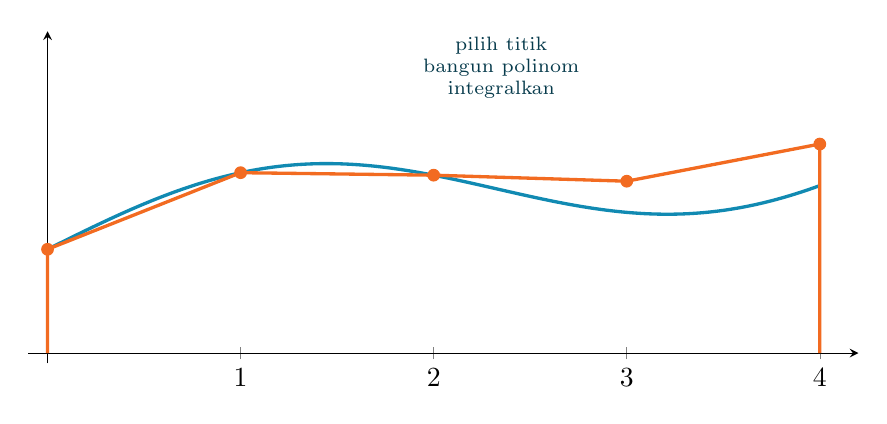
\begin{tikzpicture}
\begin{axis}[width=\linewidth,height=5.8cm,axis lines=middle,xmin=-.1,xmax=4.2,ymin=-.1,ymax=3.1,xtick={0,1,2,3,4},ytick=\empty,clip=false]
\addplot[domain=0:4,Teal,very thick,samples=160]{1.0 + .50*sin(deg(1.35*x)) + .25*x};
\addplot[only marks,mark=*,mark size=2.1pt,Orange] coordinates {(0,1.0) (1,1.738) (2,1.714) (3,1.656) (4,2.014)};
\draw[Orange,very thick] (axis cs:0,0) -- (axis cs:0,1.0) -- (axis cs:1,1.738) -- (axis cs:2,1.714) -- (axis cs:3,1.656) -- (axis cs:4,2.014) -- (axis cs:4,0);
\node[font=\scriptsize,align=center,DeepNavy] at (axis cs:2.35,2.75) {pilih titik\\bangun polinom\\integralkan};
\end{axis}
\end{tikzpicture}
\begin{orangebox}[Pertanyaan alami]
Apakah lebih banyak titik selalu lebih baik? Bagaimana jika jumlah subinterval tidak cocok dengan aturan tertentu?
\end{orangebox}
\end{column}
\end{columns}
\end{frame}

% ============ 3. LAGRANGE TO WEIGHTS ============
\begin{frame}{Bobot integral dari polinom Lagrange}
\scriptsize
\begin{columns}[T,totalwidth=\textwidth]
\begin{column}{.54\textwidth}
\begin{bluebox}[Polinom interpolasi]
Untuk titik $x_0,x_1,\ldots,x_n$,
\[
p_n(x)=\sum_{i=0}^{n} f(x_i)L_i(x),
\]
dengan
\[
L_i(x)=\prod_{\substack{j=0\\ j\ne i}}^n \frac{x-x_j}{x_i-x_j}.
\]
Jika polinom ini diintegralkan,
\[
\int_a^b p_n(x)\,dx
=\sum_{i=0}^n f(x_i)\int_a^b L_i(x)\,dx.
\]
\end{bluebox}
\end{column}
\begin{column}{.42\textwidth}
\begin{greenbox}[Makna bobot]
Koefisien pada Trapezoid, Simpson, dan Boole sebenarnya berasal dari
\[
\int L_i(x)\,dx.
\]
Jadi angka seperti $1,4,1$ atau $7,32,12,32,7$ bukan hafalan lepas, melainkan bobot area dari basis polinom.
\end{greenbox}
\begin{orangebox}[Grid seragam]
Pada Newton--Cotes, titik biasanya dipilih sama jarak:
\[
x_i=a+ih.
\]
Itulah sebabnya formula menjadi ringkas.
\end{orangebox}
\end{column}
\end{columns}
\end{frame}

% ============ 4. TRAPEZOID ============
\begin{frame}{Trapezoid: garis di antara dua ujung}
\scriptsize
\begin{columns}[T,totalwidth=\textwidth]
\begin{column}{.52\textwidth}
\begin{bluebox}[Polinom linear]
Dengan $x_0=a$, $x_1=b$,
\[
p_1(x)=f(a)+\frac{f(b)-f(a)}{b-a}(x-a).
\]
Integralkan garis tersebut pada $[a,b]$:
\[
\int_a^b p_1(x)\,dx=(b-a)\frac{f(a)+f(b)}{2}.
\]
\end{bluebox}
\begin{orangebox}[Aturan trapezoid]
\[
\boxed{I_T=(b-a)\frac{f(a)+f(b)}{2}}
\]
\end{orangebox}
\end{column}
\begin{column}{.44\textwidth}
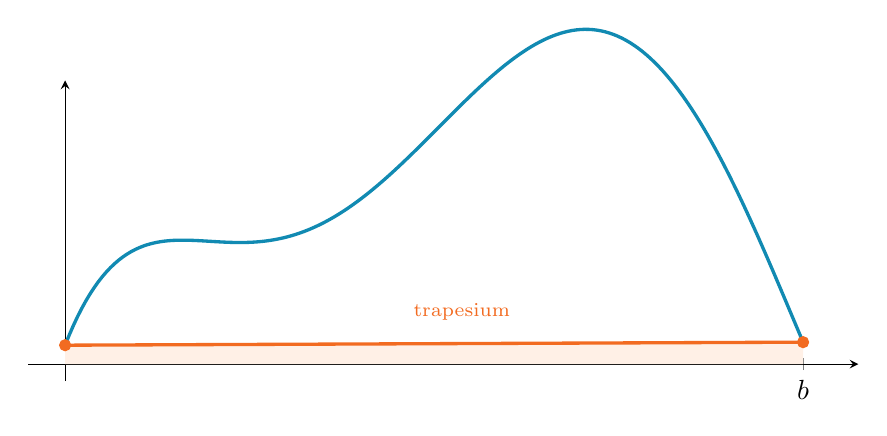
\begin{tikzpicture}
\begin{axis}[width=\linewidth,height=5.4cm,axis lines=middle,xmin=-.04,xmax=.86,ymin=-.18,ymax=3.0,xtick={0,.8},xticklabels={$a$,$b$},ytick=\empty,clip=false]
\addplot[domain=0:.8,Teal,very thick,samples=180]{0.2 + 25*x - 200*x^2 + 675*x^3 - 900*x^4 + 400*x^5};
\addplot[draw=none,fill=SoftOrange,domain=0:.8] {0.2 + .04*x} \closedcycle;
\addplot[Orange,very thick] coordinates {(0,0.2) (.8,0.232)};
\addplot[only marks,mark=*,mark size=2pt,Orange] coordinates {(0,0.2) (.8,0.232)};
\node[font=\scriptsize,Orange] at (axis cs:.43,.55) {trapesium};
\end{axis}
\end{tikzpicture}
\begin{greenbox}[Intuisi]
Kurva asli diganti garis lurus. Area di bawah garis menjadi hampiran area sejati.
\end{greenbox}
\end{column}
\end{columns}
\end{frame}

% ============ 5. COMPOSITE TRAPZ ============
\begin{frame}{Trapezoid komposit}
\scriptsize
\begin{columns}[T,totalwidth=\textwidth]
\begin{column}{.48\textwidth}
\begin{bluebox}[Banyak panel kecil]
Bagi $[a,b]$ menjadi $n$ subinterval seragam:
\[
h=\frac{b-a}{n},\qquad x_i=a+ih.
\]
Menerapkan trapezoid di setiap panel memberi
\[
\boxed{I\approx\frac{h}{2}\left[f_0+2\sum_{i=1}^{n-1}f_i+f_n\right]}.
\]
\end{bluebox}
\begin{orangebox}[Algoritma]
\begin{enumerate}\setlength\itemsep{1pt}
\item Tentukan $n$ dan $h$.
\item Hitung $x_i$ dan $f_i=f(x_i)$.
\item Bobot ujung $=1$, bobot tengah $=2$.
\item Kalikan jumlah berbobot dengan $h/2$.
\end{enumerate}
\end{orangebox}
\end{column}
\begin{column}{.48\textwidth}
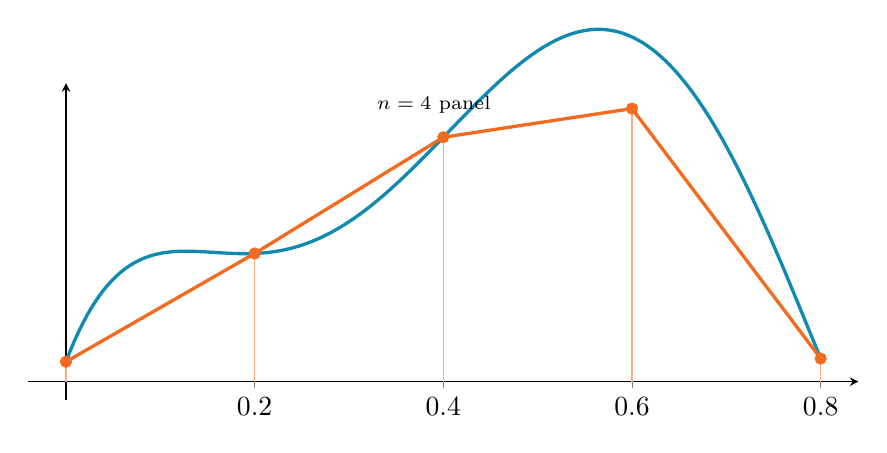
\begin{tikzpicture}
\begin{axis}[width=\linewidth,height=5.6cm,axis lines=middle,xmin=-.04,xmax=.84,ymin=-.18,ymax=3.0,xtick={0,.2,.4,.6,.8},ytick=\empty,clip=false]
\addplot[domain=0:.8,Teal,very thick,samples=180]{0.2 + 25*x - 200*x^2 + 675*x^3 - 900*x^4 + 400*x^5};
\addplot[Orange,very thick] coordinates {(0,0.2) (.2,1.288) (.4,2.456) (.6,2.744) (.8,0.232)};
\draw[Orange!55] (axis cs:0,0)--(axis cs:0,0.2);\draw[Orange!55] (axis cs:.2,0)--(axis cs:.2,1.288);\draw[Orange!55] (axis cs:.4,0)--(axis cs:.4,2.456);\draw[Orange!55] (axis cs:.6,0)--(axis cs:.6,2.744);\draw[Orange!55] (axis cs:.8,0)--(axis cs:.8,0.232);\addplot[only marks,mark=*,mark size=2pt,Orange] coordinates {(0,0.2) (.2,1.288) (.4,2.456) (.6,2.744) (.8,0.232)};
\node[font=\scriptsize] at (axis cs:.39,2.78) {$n=4$ panel};
\end{axis}
\end{tikzpicture}
\begin{greenbox}[Pola bobot]
\[
1,\ 2,\ldots,2,\ 1
\]
Ujung dihitung sekali, titik interior muncul dari dua panel.
\end{greenbox}
\end{column}
\end{columns}
\end{frame}

% ============ 6. SIMPSON 1/3 ============
\begin{frame}{Simpson 1/3: parabola dari tiga titik}
\scriptsize
\begin{columns}[T,totalwidth=\textwidth]
\begin{column}{.54\textwidth}
\begin{bluebox}[Bangun parabola]
Ambil tiga titik berjarak sama:
\[
x_0=a,\qquad x_1=a+h,\qquad x_2=a+2h=b.
\]
Gunakan
\[
p_2(x)=f_0L_0(x)+f_1L_1(x)+f_2L_2(x).
\]
Dengan $x=x_0+sh$ dan $s\in[0,2]$,
\[
\int_0^2 L_0(s)ds=\frac13,
\quad \int_0^2 L_1(s)ds=\frac43,
\quad \int_0^2 L_2(s)ds=\frac13.
\]
\end{bluebox}
\begin{orangebox}[Formula]
\[
\boxed{I_{1/3}\approx \frac{h}{3}\left(f_0+4f_1+f_2\right)}
\]
Disebut $1/3$ karena muncul faktor $h/3$.
\end{orangebox}
\end{column}
\begin{column}{.42\textwidth}
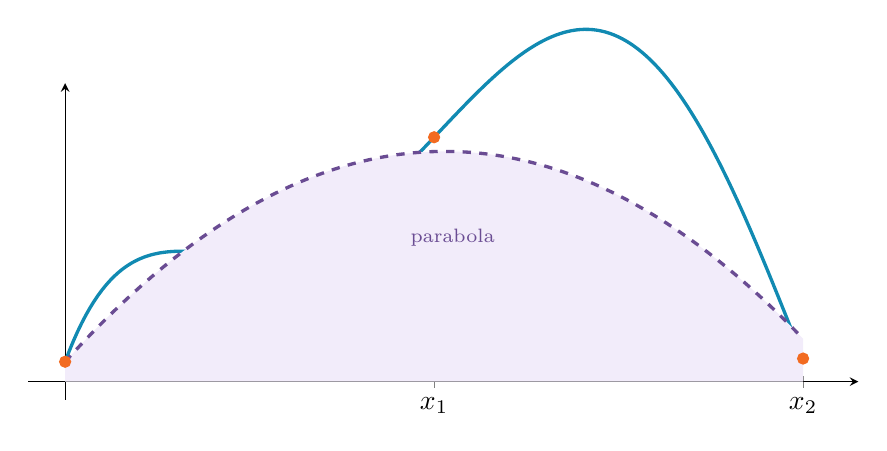
\begin{tikzpicture}
\begin{axis}[width=\linewidth,height=5.6cm,axis lines=middle,xmin=-.04,xmax=.86,ymin=-.18,ymax=3.0,xtick={0,.4,.8},xticklabels={$x_0$,$x_1$,$x_2$},ytick=\empty,clip=false]
\addplot[domain=0:.8,Teal,very thick,samples=180]{0.2 + 25*x - 200*x^2 + 675*x^3 - 900*x^4 + 400*x^5};
\addplot[draw=none,fill=SoftPurple,domain=0:.8,samples=120]{0.2+10.2726666667*x-12.48*x^2} \closedcycle;
\addplot[Purple,very thick,dashed,domain=0:.8,samples=120]{0.2+10.2726666667*x-12.48*x^2};
\addplot[only marks,mark=*,mark size=2pt,Orange] coordinates {(0,0.2) (.4,2.456) (.8,0.232)};
\node[font=\scriptsize,Purple] at (axis cs:.42,1.45) {parabola};
\end{axis}
\end{tikzpicture}
\begin{greenbox}[Dibanding Trapezoid]
Satu titik tengah membuat kurva lokal ditangkap lebih baik daripada garis lurus.
\end{greenbox}
\end{column}
\end{columns}
\end{frame}

% ============ 7. SIMPSON 1/3 COMPOSITE ============
\begin{frame}{Simpson 1/3 komposit}
\scriptsize
\begin{columns}[T,totalwidth=\textwidth]
\begin{column}{.54\textwidth}
\begin{bluebox}[Banyak parabola]
Simpson $1/3$ memakai dua subinterval per panel. Karena itu, kompositnya membutuhkan $n$ \highlight{genap}.
\[
I\approx \frac{h}{3}\left[f_0+4\sum_{i=1,3,5}^{n-1}f_i+2\sum_{i=2,4,6}^{n-2}f_i+f_n\right].
\]
\end{bluebox}
\begin{orangebox}[Pola bobot]
\[
1,
4,
2,
4,
2,
\ldots,
4,
1.
\]
Bobot $4$ berada pada titik tengah tiap panel parabola.
\end{orangebox}
\end{column}
\begin{column}{.42\textwidth}
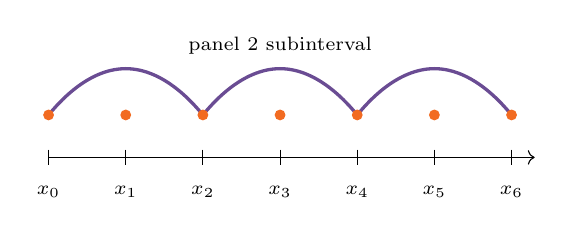
\begin{tikzpicture}[scale=.98]
\draw[->] (0,0) -- (6.3,0);
\foreach \x/\lab in {0/$x_0$,1/$x_1$,2/$x_2$,3/$x_3$,4/$x_4$,5/$x_5$,6/$x_6$}{\draw (\x,.1)--(\x,-.1) node[below=4pt,font=\scriptsize]{\lab};}
\draw[Purple,very thick] (0,.55) parabola bend (1,1.15) (2,.55);
\draw[Purple,very thick] (2,.55) parabola bend (3,1.15) (4,.55);
\draw[Purple,very thick] (4,.55) parabola bend (5,1.15) (6,.55);
\foreach \x in {0,1,2,3,4,5,6}{\fill[Orange] (\x,.55) circle (2pt);}
\node[font=\scriptsize] at (3,1.45) {panel 2 subinterval};
\end{tikzpicture}
\vspace{2mm}
\begin{greenbox}[Kapan dipakai?]
Jika jumlah subinterval genap dan data cukup halus, Simpson $1/3$ biasanya menjadi pilihan utama.
\end{greenbox}
\end{column}
\end{columns}
\end{frame}

% ============ 8. SIMPSON 3/8 ============
\begin{frame}{Simpson 3/8: empat titik, tiga subinterval}
\scriptsize
\begin{columns}[T,totalwidth=\textwidth]
\begin{column}{.52\textwidth}
\begin{purplebox}[Polinom kubik]
Ambil empat titik berjarak sama:
\[
x_0,x_1,x_2,x_3,
\qquad h=\frac{b-a}{3}.
\]
Polinom kubik $p_3(x)$ yang melewati empat titik diintegralkan pada $[x_0,x_3]$:
\[
\boxed{I_{3/8}\approx\frac{3h}{8}(f_0+3f_1+3f_2+f_3)}.
\]
Disebut $3/8$ karena faktor di depan bobotnya $3h/8$.
\end{purplebox}
\begin{goldbox}[Kapan muncul?]
Jika jumlah subinterval ganjil, Simpson $1/3$ tidak dapat menutup semua panel. Ambil sebanyak mungkin Simpson $1/3$, lalu gunakan satu blok Simpson $3/8$ untuk tiga subinterval terakhir.
\end{goldbox}
\end{column}
\begin{column}{.44\textwidth}
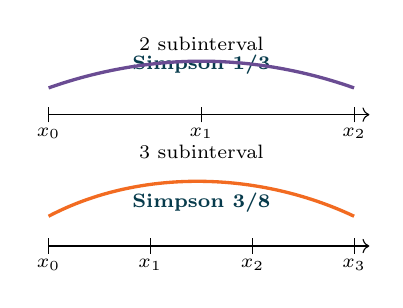
\begin{tikzpicture}[scale=.97]
\node[font=\bfseries\scriptsize,DeepNavy] at (2,1.75) {Simpson 1/3};
\draw[->] (0,1.1) -- (4.2,1.1);
\foreach \x/\lab in {0/$x_0$,2/$x_1$,4/$x_2$}{\draw (\x,1.0)--(\x,1.2) node[below=4pt,font=\scriptsize]{\lab};}
\draw[Purple,very thick] (0,1.45) parabola bend (2,1.80) (4,1.45);
\node[font=\scriptsize] at (2,2.03) {2 subinterval};
\node[font=\bfseries\scriptsize,DeepNavy] at (2,-.05) {Simpson 3/8};
\draw[->] (0,-.62) -- (4.2,-.62);
\foreach \x/\lab in {0/$x_0$,1.33/$x_1$,2.67/$x_2$,4/$x_3$}{\draw (\x,-.72)--(\x,-.52) node[below=4pt,font=\scriptsize]{\lab};}
\draw[Orange,very thick] (0,-.23) .. controls (1.2,.40) and (2.75,.36) .. (4,-.23);
\node[font=\scriptsize] at (2,.62) {3 subinterval};
\end{tikzpicture}
\begin{greenbox}[Aturan cepat]
$n$ genap: Simpson $1/3$.\quad
$n$ ganjil: kombinasi $1/3$ dan $3/8$.
\end{greenbox}
\end{column}
\end{columns}
\end{frame}

% ============ 9. BOOLE ============
\begin{frame}{Aturan Boole: lima titik dalam satu panel}
\scriptsize
\begin{columns}[T,totalwidth=\textwidth]
\begin{column}{.50\textwidth}
\begin{bluebox}[Polinom kuartik]
Boole memakai lima titik berjarak sama:
\[
x_0,x_1,x_2,x_3,x_4,
\qquad h=\frac{b-a}{4}.
\]
Polinom derajat empat diintegralkan pada $[x_0,x_4]$:
\[
\boxed{I_B\approx\frac{2h}{45}\left(7f_0+32f_1+12f_2+32f_3+7f_4\right)}.
\]
Setara dengan
\[
\frac{b-a}{90}(7f_0+32f_1+12f_2+32f_3+7f_4).
\]
\end{bluebox}
\end{column}
\begin{column}{.46\textwidth}
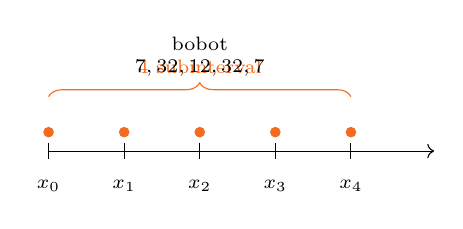
\begin{tikzpicture}[scale=.96]
\draw[->] (0,0) -- (5.1,0);
\foreach \x/\lab in {0/$x_0$,1/$x_1$,2/$x_2$,3/$x_3$,4/$x_4$}{\draw (\x,.11)--(\x,-.11) node[below=4pt,font=\scriptsize]{\lab};}
\draw[Orange,decorate,decoration={brace,amplitude=5pt}] (0,.72)--(4,.72) node[midway,above=5pt,font=\scriptsize] {4 subinterval};
\foreach \x in {0,1,2,3,4}{\fill[Orange] (\x,.25) circle (2pt);}
\node[font=\scriptsize,align=center] at (2,1.25) {bobot\\$7,32,12,32,7$};
\end{tikzpicture}
\begin{orangebox}[Karakter]
\begin{itemize}\setlength\itemsep{1pt}
\item Memakai 4 subinterval per panel.
\item Bobot simetris.
\item Cocok untuk fungsi halus pada grid seragam.
\end{itemize}
\end{orangebox}
\begin{greenbox}[Urutan ide]
Trapezoid: garis.\quad Simpson: parabola/kubik.\quad Boole: kuartik.
\end{greenbox}
\end{column}
\end{columns}
\end{frame}

% ============ 10. HOW TO CHOOSE ============
\begin{frame}{Memilih aturan pada grid seragam}
\scriptsize
\begin{columns}[T,totalwidth=\textwidth]
\begin{column}{.52\textwidth}
\begin{greenbox}[Panel dan syarat]
\begin{tabular}{lcc}
\toprule
Aturan & Titik/panel & Subinterval/panel\\\midrule
Trapezoid & 2 & 1\\
Simpson $1/3$ & 3 & 2\\
Simpson $3/8$ & 4 & 3\\
Boole & 5 & 4\\
\bottomrule
\end{tabular}
\end{greenbox}
\begin{orangebox}[Strategi]
\begin{itemize}\setlength\itemsep{1pt}
\item Jika $n$ genap: Simpson $1/3$ komposit.
\item Jika $n$ ganjil dan $n\ge3$: gunakan Simpson $1/3$ untuk bagian genap, lalu Simpson $3/8$ untuk tiga subinterval terakhir.
\item Boole dipakai jika panel 4 subinterval tersedia dan fungsi cukup halus.
\end{itemize}
\end{orangebox}
\end{column}
\begin{column}{.44\textwidth}
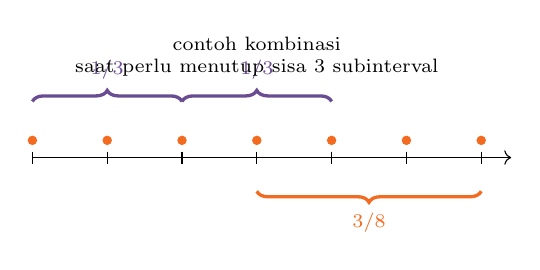
\begin{tikzpicture}[scale=.95]
\draw[->] (0,0) -- (6.4,0);
\foreach \x in {0,1,2,3,4,5,6}{\draw (\x,.08)--(\x,-.08); \fill[Orange] (\x,.23) circle (1.8pt);}
\draw[Purple,very thick,decorate,decoration={brace,amplitude=4pt}] (0,.75)--(2,.75) node[midway,above=4pt,font=\scriptsize]{1/3};
\draw[Purple,very thick,decorate,decoration={brace,amplitude=4pt}] (2,.75)--(4,.75) node[midway,above=4pt,font=\scriptsize]{1/3};
\draw[Orange,very thick,decorate,decoration={brace,amplitude=4pt,mirror}] (3,-.45)--(6,-.45) node[midway,below=4pt,font=\scriptsize]{3/8};
\node[font=\scriptsize,align=center] at (3,1.35) {contoh kombinasi\\saat perlu menutup sisa 3 subinterval};
\end{tikzpicture}
\begin{bluebox}[Catatan]
Pemilihan aturan bukan sekadar rumus; harus cocok dengan jumlah titik, jarak titik, dan kehalusan fungsi.
\end{bluebox}
\end{column}
\end{columns}
\end{frame}

% ============ 11. EXAMPLE ============
\begin{frame}{Contoh dengan pembanding analitik}
\scriptsize
\begin{columns}[T,totalwidth=\textwidth]
\begin{column}{.52\textwidth}
\begin{bluebox}[Fungsi uji]
\[
f(x)=0.2+25x-200x^2+675x^3-900x^4+400x^5,
\quad 0\le x\le0.8.
\]
Integral analitiknya
\[
F(x)=0.2x+\frac{25}{2}x^2-\frac{200}{3}x^3+\frac{675}{4}x^4-180x^5+\frac{400}{6}x^6.
\]
\[
I_{\rm exact}=F(0.8)-F(0)=1.640533.
\]
\end{bluebox}
\end{column}
\begin{column}{.44\textwidth}
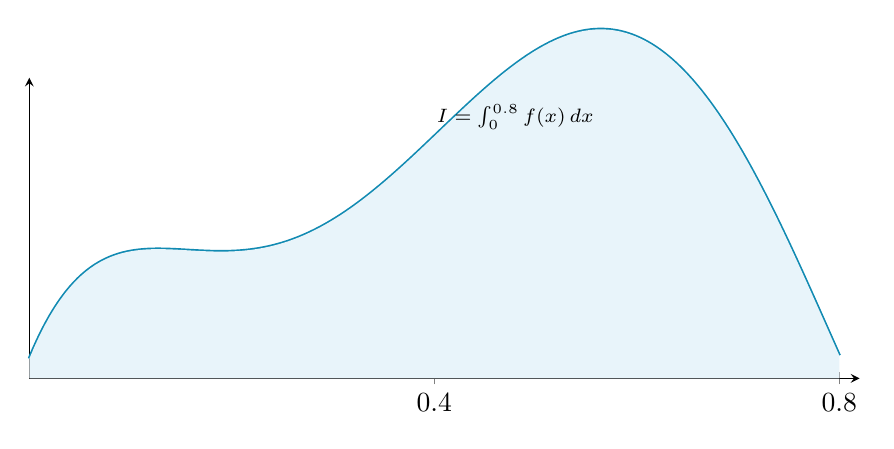
\begin{tikzpicture}
\begin{axis}[width=\linewidth,height=5.4cm,axis lines=middle,xmin=0,xmax=.82,ymin=0,ymax=3.05,xtick={0,.4,.8},ytick=\empty,clip=false]
\addplot[domain=0:.8,Teal,very thick,samples=200]{0.2 + 25*x - 200*x^2 + 675*x^3 - 900*x^4 + 400*x^5};
\addplot[draw=none,fill=SoftBlue,domain=0:.8,samples=160]{0.2 + 25*x - 200*x^2 + 675*x^3 - 900*x^4 + 400*x^5} \closedcycle;
\node[font=\scriptsize] at (axis cs:.48,2.65) {$I=\int_0^{0.8} f(x)\,dx$};
\end{axis}
\end{tikzpicture}
\begin{orangebox}[Ukuran galat]
\[
e_r=\left|\frac{I_{\rm exact}-I_{\rm num}}{I_{\rm exact}}\right|\times100\%.
\]
\end{orangebox}
\end{column}
\end{columns}
\end{frame}

% ============ 12. RESULTS ============
\begin{frame}{Membaca hasil beberapa aturan}
\scriptsize
\begin{columns}[T,totalwidth=\textwidth]
\begin{column}{.50\textwidth}
\begin{greenbox}[Beberapa nilai]
\begin{tabular}{lcc}
\toprule
Aturan & Nilai & Pola galat\\\midrule
Trapezoid tunggal & $0.172800$ & besar\\
Trapezoid $n=2$ & $1.068800$ & turun\\
Simpson $1/3$ tunggal & $1.367467$ & lebih dekat\\
Simpson $1/3$, $n=4$ & $1.623467$ & dekat\\
\bottomrule
\end{tabular}
\end{greenbox}
\begin{orangebox}[Interpretasi]
Memperkecil panel biasanya memperbaiki hasil. Mengganti garis dengan polinom orde lebih tinggi juga dapat memperbaiki hasil, selama fungsi cukup halus dan grid cocok.
\end{orangebox}
\end{column}
\begin{column}{.46\textwidth}
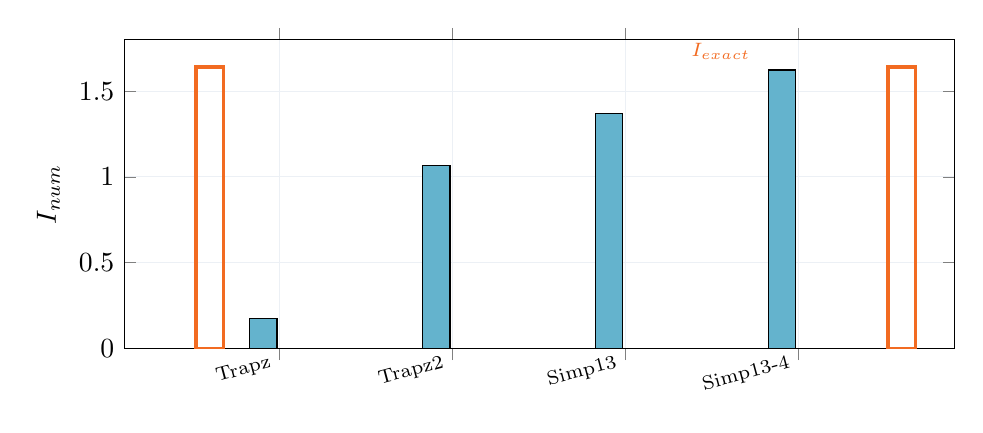
\begin{tikzpicture}
\begin{axis}[width=\linewidth,height=5.5cm,ybar,bar width=10pt,ymin=0,ymax=1.8,xtick=data,xticklabels={Trapz,Trapz2,Simp13,Simp13-4},x tick label style={font=\scriptsize,rotate=15,anchor=east},ylabel={$I_{num}$},grid=major,grid style={LightLine!50}]
\addplot[fill=Teal!65] coordinates {(1,0.1728) (2,1.0688) (3,1.367467) (4,1.623467)};
\addplot[Orange,very thick,domain=.5:4.5,samples=2] {1.640533};
\node[font=\scriptsize,Orange] at (axis cs:3.55,1.73) {$I_{exact}$};
\end{axis}
\end{tikzpicture}
\end{column}
\end{columns}
\end{frame}

% ============ 13. ALGORITHM ============
\begin{frame}{Algoritma umum Newton--Cotes komposit}
\scriptsize
\begin{columns}[T,totalwidth=\textwidth]
\begin{column}{.52\textwidth}
\begin{bluebox}[Langkah komputasi]
\begin{enumerate}\setlength\itemsep{3pt}
\item Tentukan interval $[a,b]$ dan jumlah subinterval $n$.
\item Hitung $h=(b-a)/n$ dan titik $x_i=a+ih$.
\item Hitung $f_i=f(x_i)$.
\item Pilih pola bobot sesuai aturan.
\item Hitung $I\approx h\sum w_i f_i$.
\item Jika pembanding tersedia, hitung galat.
\end{enumerate}
\end{bluebox}
\end{column}
\begin{column}{.44\textwidth}
\begin{orangebox}[Pola bobot]
\begin{tabular}{lc}
\toprule
Aturan & Bobot lokal\\\midrule
Trapezoid & $\frac12[1,1]$\\
Simpson $1/3$ & $\frac13[1,4,1]$\\
Simpson $3/8$ & $\frac38[1,3,3,1]$\\
Boole & $\frac{2}{45}[7,32,12,32,7]$\\
\bottomrule
\end{tabular}
\end{orangebox}
\begin{greenbox}[Function--driver]
Simpan aturan sebagai function, lalu driver cukup memilih fungsi, interval, $n$, serta grafik yang ingin dibaca.
\end{greenbox}
\end{column}
\end{columns}
\end{frame}

% ============ 14. MATLAB ============
\begin{frame}[fragile]{Demo MATLAB ringkas}
\scriptsize
\begin{columns}[T,totalwidth=\textwidth]
\begin{column}{.55\textwidth}
\begin{bluebox}[Driver]
\begin{verbatim}
f = @(x) 0.2 + 25*x - 200*x.^2 + 675*x.^3 ...
         - 900*x.^4 + 400*x.^5;
a = 0; b = 0.8; n = 4;
I = simpson13_comp(f,a,b,n);
F = @(x) 0.2*x + 25/2*x.^2 - 200/3*x.^3 ...
         + 675/4*x.^4 - 180*x.^5 + 400/6*x.^6;
Iexact = F(b)-F(a);
err = abs(I-Iexact)/abs(Iexact);
\end{verbatim}
\end{bluebox}
\end{column}
\begin{column}{.41\textwidth}
\begin{orangebox}[Function]
\begin{verbatim}
function I = simpson13_comp(f,a,b,n)
    if mod(n,2) ~= 0
        error('n harus genap')
    end
    h = (b-a)/n;
    x = a:h:b;
    y = f(x);
    I = h/3*(y(1) + 4*sum(y(2:2:end-1)) ...
             + 2*sum(y(3:2:end-2)) + y(end));
end
\end{verbatim}
\end{orangebox}
\end{column}
\end{columns}
\end{frame}

% ============ 15. GRAPH ERROR ============
\begin{frame}{Melihat konvergensi integral}
\scriptsize
\begin{columns}[T,totalwidth=\textwidth]
\begin{column}{.46\textwidth}
\begin{bluebox}[Eksperimen numerik]
Coba beberapa $n$ yang sesuai:
\[
n=2,4,8,16,32.
\]
Untuk tiap $n$, hitung $I_n$ dan galat relatif. Jika metode konsisten, galat akan turun ketika panel diperkecil.
\end{bluebox}
\begin{orangebox}[Yang diamati]
\begin{itemize}\setlength\itemsep{1pt}
\item nilai integral,
\item galat terhadap analitik,
\item grafik galat terhadap $h$ atau $n$,
\item aturan mana yang paling efisien.
\end{itemize}
\end{orangebox}
\end{column}
\begin{column}{.50\textwidth}
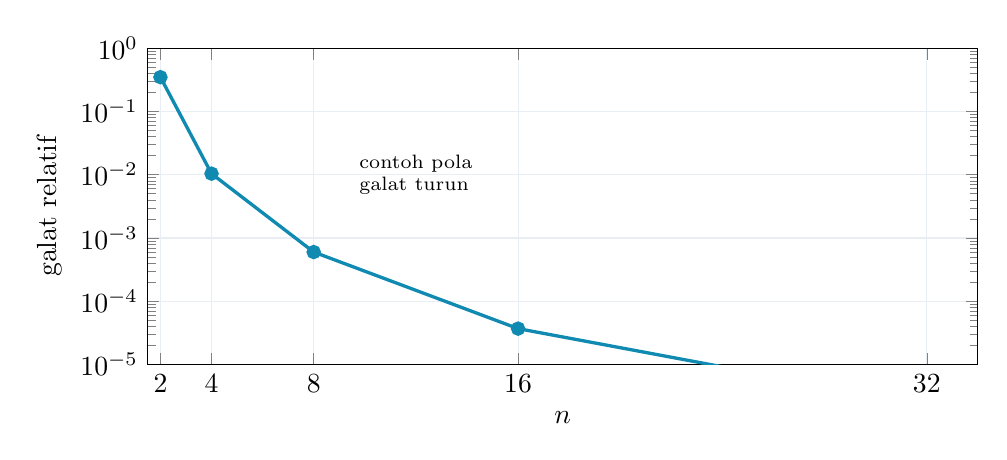
\begin{tikzpicture}
\begin{semilogyaxis}[width=\linewidth,height=5.6cm,xlabel={$n$},ylabel={galat relatif},xmin=1.5,xmax=34,ymin=1e-5,ymax=1,grid=major,grid style={LightLine!60},xtick={2,4,8,16,32}]
\addplot[Teal,very thick,mark=*] coordinates {(2,3.48e-1) (4,1.04e-2) (8,6.0e-4) (16,3.7e-5) (32,2.3e-6)};
\node[font=\scriptsize,align=left] at (axis cs:12,1e-2) {contoh pola\\galat turun};
\end{semilogyaxis}
\end{tikzpicture}
\end{column}
\end{columns}
\end{frame}

% ============ 16. ODE CASE ============
\begin{frame}{Case: integral numerik untuk PDB separabel}
\scriptsize
\begin{columns}[T,totalwidth=\textwidth]
\begin{column}{.50\textwidth}
\begin{bluebox}[Ketika PDB berubah menjadi integral]
Tidak semua PDB dapat langsung diselesaikan dengan integral numerik. Bentuk yang cocok misalnya
\[
\frac{dy}{dt}=g(t),\qquad y(0)=y_0.
\]
Maka
\[
y(T)=y_0+\int_0^T g(t)\,dt.
\]
Jika $g(t)$ rumit atau hanya tersedia sebagai data, integralnya dapat dihampiri dengan Newton--Cotes.
\end{bluebox}
\begin{orangebox}[Contoh]
\[
\frac{dy}{dt}=e^{-t^2},\qquad y(0)=1.
\]
\[
y(1)=1+\int_0^1 e^{-t^2}\,dt.
\]
\end{orangebox}
\end{column}
\begin{column}{.46\textwidth}
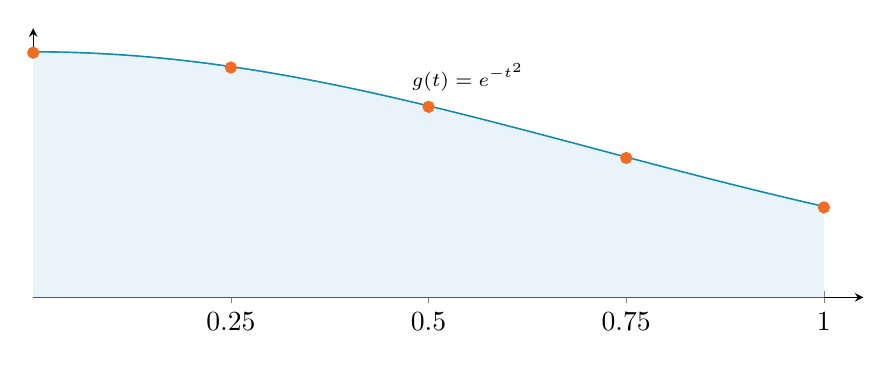
\begin{tikzpicture}
\begin{axis}[width=\linewidth,height=5.0cm,axis lines=middle,xmin=0,xmax=1.05,ymin=0,ymax=1.1,xtick={0,.25,.5,.75,1},ytick=\empty,clip=false]
\addplot[domain=0:1,Teal,very thick,samples=120]{exp(-x^2)};
\addplot[draw=none,fill=SoftBlue,domain=0:1,samples=120]{exp(-x^2)} \closedcycle;
\addplot[only marks,Orange,mark=*] coordinates {(0,1) (.25,.9394) (.5,.7788) (.75,.5698) (1,.3679)};
\node[font=\scriptsize] at (axis cs:.55,.90) {$g(t)=e^{-t^2}$};
\end{axis}
\end{tikzpicture}
\begin{greenbox}[Dengan Simpson 1/3 n=4]
\[
\int_0^1 e^{-t^2}dt\approx0.746855.
\]
Sehingga
\[
y(1)\approx1.746855.
\]
\end{greenbox}
\end{column}
\end{columns}
\end{frame}

% ============ 17. EXERCISES ============
\begin{frame}{Latihan}
\scriptsize
\begin{orangebox}[1. Dasar]
Gunakan Trapezoid tunggal, Trapezoid komposit $n=2$, Simpson $1/3$ tunggal, dan Simpson $1/3$ komposit $n=4$ untuk
\[
f(x)=0.2+25x-200x^2+675x^3-900x^4+400x^5.
\]
Bandingkan dengan integral analitiknya.
\end{orangebox}
\begin{greenbox}[2. Pemilihan aturan]
Untuk grid seragam dengan $n=5$ subinterval, jelaskan kombinasi Simpson $1/3$ dan Simpson $3/8$ yang masuk akal. Terapkan pada fungsi yang sama.
\end{greenbox}
\begin{purplebox}[3. PDB separabel]
Hitung
\[
y(1)=1+\int_0^1 e^{-t^2}\,dt
\]
dengan Trapezoid komposit, Simpson $1/3$ komposit, dan Boole. Buat grafik galat terhadap jumlah subinterval jika tersedia pembanding numerik yang sangat halus.
\end{purplebox}
\end{frame}

\end{document}
